% EPC flow charts
% Author: Fabian Schuh
\documentclass{article}
\usepackage{myflowchart}
\usepackage{verbatim}
\usepackage{standalone}
%\usepackage{tikz}
\usepackage{menukeys}

\newmenumacro{\nixfile}[/]{hyphenatepaths}
\newmenumacro{\nixpath}[/]{hyphenatepathswithfolder}
\newmenumacro{\winpath}[bslash]{hyphenatepathswithfolder}
\newmenumacro{\winfile}[bslash]{hyphenatepaths}

\begin{document}

\begin{tikzpicture}

\begin{scope}[node distance=5mm and 5mm]

\node [ item=4](a) at (1,1) {%
            \textbf{擴充}
            \nodepart{two}
            \begin{enumerate}
            	\item gyro sensor轉動驗證,準確性歸納。應用?
		\item 兵乓球轉動積分器檢查。$\circ\circ\circ$
		\item 易德問$\omega_b$証。
		\item GUI照note中Fig 7下方的手寫紀錄來分類,照獨自子題,不要想統合了。
            	\item 結合疊格來做立體作圖?first do proof of concept. $\circ\circ\circ$
            	\item 增加藍芽傳輸(沒有wifi時)
            	\item 與ejss準確度比較
            	\item 偏移誤差近似與改進(與ejss,sensor轉動驗證均有關係)
            	\item 加光線追蹤美觀化?換白色cube?
            	\item unity3D飛機滑鼠控制器?與race simulation屬同性質demo。
           \end{enumerate}
           \nodepart{three}\textbf{待修正事項}
	\nodepart{four}
	\begin{enumerate}
            \item GUI設計卡住,見第二頁討論
            \item OpenGL animation關閉後要手動重啟一個新個interpreter,因為glut的關係,怎麼改進?
            \item py2exe作業系統可執行檔,軟體化
            \item mplot3D例子全換OpenGL?
            \item OpenGL動畫延遲,不能漏接貼角。
            \item 製作gimbal中...
	\end{enumerate}
            };

\node [gitrec,below=of a](b)   
{git log}edge [<-,>=stealth'] (a);

\node [item=2,below=of b](c)
{%
\textbf{模擬軟體擴充}
\nodepart{two}
\begin{enumerate}
            \item 增加新模擬,包括物理引擎python與OpenGL動畫呈現。動畫物體的繪製也很花時間。
            \item 寫程式函式說明,update演進紀錄changelog,(comment \& documentation \& update log)
            \item 用py2exe調整做成exe
\end{enumerate}
}edge [<-,>=stealth'] (b);

\node [gitrec,below=of c](d)   
{git log}edge [<-,>=stealth'] (c);

\node [above right = of a.north east, align=center, anchor = south] (title){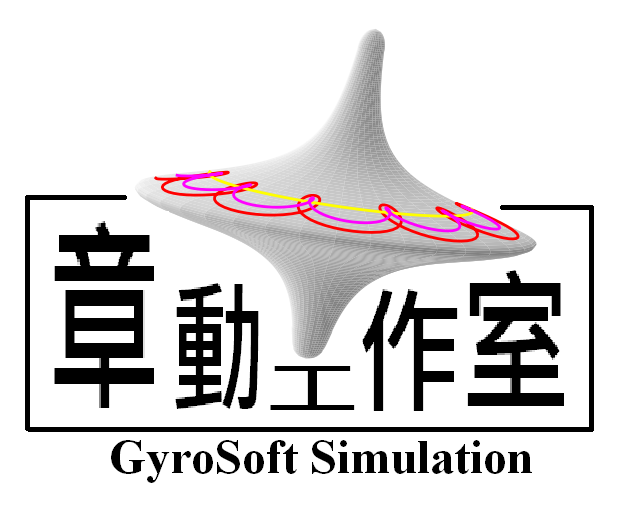
\includegraphics[width=0.4\textwidth]{../../figs/test_new_logo_chinese.png}\\ \LARGE 作業流程};

\node [item=2,below right = of title.south, anchor = north west ](e)
{%
\textbf{pdf文件}
\nodepart{two}
\begin{enumerate}
            \item 製作要放入文件的圖片(疊格技術運用)
            \item 以MacKichan Scientific Word軟體撰寫擴充的新內容,寫軟體操作說明,然後使用本工作室開發的自動化流程來進行章節或全書的編譯(使用Xelatex引擎),來產生PDF技術文件。
            \item 列印,技術文件裝訂成冊
\end{enumerate}
};%edge [<-,>=stealth'] (d);

%draw the curve line
%\draw [->,out = 180, in = 0] (h) to  (f);



\node [phantom, left=of e](gic2){};
\node [phantom, below right=of c](gic1){};

\node [gitrec,below=of e](f){git log}edge [<-,>=stealth'] (e);

\node [item=2,below = of f](g)
{\textbf{加入網頁}
\nodepart{two}
\begin{enumerate}
            \item 製作網頁可觀看的示範影片
            \item Landing page的修改。以LYX增加Landing page的新內容,然後利用LYX的HTML export功能,若有數學要加上使用Mathjax的選項。然後git push上pyanywere網站。
            \item 有時也需要把技術文件po上網頁,做成blog文章,此時就利用SW中的export HTML功能。需要時要微調。例如production chapter。
\end{enumerate}
}edge [<-,>=stealth'] (f);

\draw [rounded corners,->,>=stealth'] (d) --  (gic1.center) -- (gic2.center) -- (e);


\node [item=2,below=of g](h)
{%
\textbf{推廣(找專人負責)}
\nodepart{two}
\begin{enumerate}
            \item 陀螺儀應用體驗店
            \item 廣告文宣製作,以landing page製作flyer。將LYX中landing page的內容export成xetex碼,然後在texlive按照我們整理好的方式修改成Texlive的xelatex可編譯碼,然後編譯成PDF flyer。列印後發放。
            \item gss logo不同型式的製作,名片電繡等製作。
\end{enumerate}
}edge [<-,>=stealth'] (g);


\end{scope}
\end{tikzpicture}

% second page
\begin{tikzpicture}[item]
\begin{scope}[node distance=5mm and 5mm]

\node [ item=2](tree) at (1,1) {%
            \textbf{GS軟體資料夾一覽}
            \nodepart[text width = 8.2cm]{two}
	    \documentclass{standalone}

\usepackage{menukeys}

\newmenumacro{\nixfile}[/]{hyphenatepaths}
\newmenumacro{\nixpath}[/]{hyphenatepathswithfolder}
\newmenumacro{\winpath}[bslash]{hyphenatepathswithfolder}
\newmenumacro{\winfile}[bslash]{hyphenatepaths}

\begin{document}
\begin{minipage}{\textwidth}
\begin{tabbing}
\hspace{1em}\=\hspace{1em}\=\hspace{1em}\=\hspace{1em}\=\\\kill
%\nixpath{Demo\_Examples }                            \\
%\>\nixpath{spinning\_top\_gyroscope}       	     \\
%\>\>\nixpath{four\_classical\_motions\_demo} 	     \\
%\>\>\>\nixpath{OpenGL\_animation} 	     \\
%\>\>\>\>\nixfile{cusp\_GL.py}    			     \\
%\>\nixpath{RigidBody\_rotation\_integrator}	     \\
%\>\nixpath{MEMS\_gyro\_sensor} 			\\
%\nixfile{subfile   } 						  \\
%\nixfile{wierd/file}   \\
%\nixfile{file      }\\
%\nixpath{four\_classical\_motions\_demo/}    \\
%\>\nixpath{OpenGL\_animation/}    \\
%\>\>\nixfile{circle\_GL.py}    \\
%\>\>\nixfile{circle\_GL\_with\_B\_method.py}    \\
%\>\>\nixfile{curly\_ring\_GL.py}    \\
%\>\>\nixfile{cusp\_GL.py}    \\
%\>\>\nixfile{wave\_like\_GL.py}    \\
%\>\nixpath{python\_animation/}    \\
%\>\>\nixfile{circle.py}    \\
%\>\>\nixfile{curly\_ring.py}    \\
%\>\>\nixfile{cusp.py}    \\
%\>\>\nixfile{wave\_like.py}    \\
\nixpath{Demo\_Examples/}\\
\>\nixfile{ReadMe.txt}\\
\>\nixfile{User\_interface.py}\\
\>\nixpath{GUIs/}\\
\>\>\nixfile{GUI\_test.py}\\
\>\>\nixfile{GUI\_TryMe\_v3.py}\\
\>\>\nixfile{GUI\_TryMe\_v4.py}\\
\>\>\nixfile{GUI\_TryMe\_v5.py}\\
\>\nixpath{mechanical\_gyro\_design/}\\
\>\>\nixfile{centripetal\_mass\_spring.py}\\
\>\nixpath{MEMS\_gyro\_sensor/}\\
\>\>\nixfile{Gyro\_Ring\_Test.py}\\
\>\>\nixfile{MEMSinVR\_demo.py}\\
\>\>\nixfile{MEMS\_rotation\_control\_in\_python.py}\\
\>\>\nixfile{NoisyTest.py}\\
\>\>\nixfile{StillTest.py}\\
\>\nixpath{RigidBody\_rotation\_integrator/}\\
\>\>\nixfile{gyro\_ring\_test\_1.py}\\
\>\>\nixfile{pingpong.py}\\
\>\>\nixfile{pingpong\_2.py}\\
\>\>\nixfile{self\_energized.py}\\
\>\>\nixfile{self\_energized\_check\_Lcentering.py}\\
\>\nixpath{spinning\_top\_gyroscope/}\\
\>\>\nixfile{F\_contact\_force.py}\\
\>\>\nixfile{Gyroscope-TeachDemo-custumed\_parameters.py}\\
\>\>\nixfile{Gyroscope\_SpaceBodyCone.py}\\
\>\>\nixfile{Hercules\_explain.py}\\
\>\>\nixfile{L\_not\_circle.py}\\
\>\>\nixfile{Spinning\_cube\_swinging\_under\_g\_with\_gyroscopic\_effect.py}\\
\>\>\nixpath{comparing\_integration\_methods/}\\
\>\>\>\nixfile{AngularVelocityTrail\_in\_body\_frame\_compare\_ABmethods.py}\\
\>\>\nixpath{four\_classical\_motions\_demo/}\\
\>\>\>\nixpath{OpenGL\_animation/}\\
\>\>\>\>\nixfile{circle\_GL.py}\\
\>\>\>\>\nixfile{circle\_GL\_with\_B\_method.py}\\
\>\>\>\>\nixfile{curly\_ring\_GL.py}\\
\>\>\>\>\nixfile{cusp\_GL.py}\\
\>\>\>\>\nixfile{wave\_like\_GL.py}\\
\>\>\>\nixpath{python\_animation/}\\
\>\>\>\>\nixfile{circle.py}\\
\>\>\>\>\nixfile{curly\_ring.py}\\
\>\>\>\>\nixfile{cusp.py}\\
\>\>\>\>\nixfile{wave\_like.py}\\
\end{tabbing}
\end{minipage}
\end{document}

	    };

\node [above right = of tree.north east, align=center, anchor = south] (title2){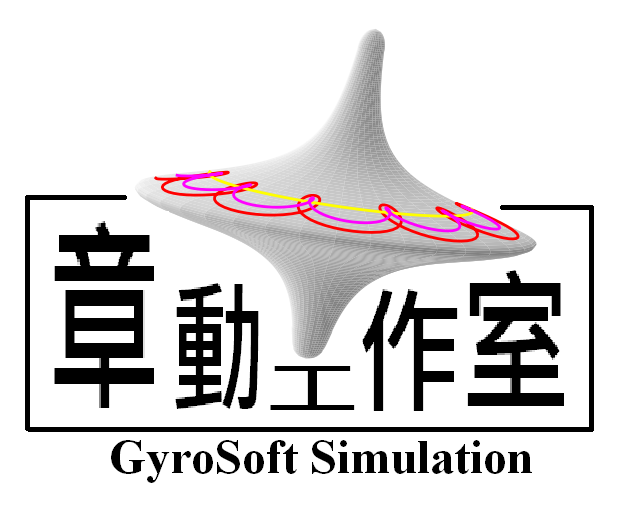
\includegraphics[width=0.6\textwidth]{../../figs/test_new_logo_chinese.png}};
%\parbox[c][][c]{0.3\textwidth}{}
%\parbox[c][][c]{5cm}{\Huge 卡住kazoo}
\node [ item=2, below right = of title2.south, anchor = north west](gitlog) {%
            \textbf{last 10 git commits}
            \nodepart[text width = 8.2cm]{two}
	    \footnotesize \verbatiminput{log.log}
	    };

\end{scope}
\end{tikzpicture}
% end second page

% third page
\begin{tikzpicture}[item]
\begin{scope}[node distance=5mm and 5mm]

\node [ item=2](thinking) at (1,1) {%
            \textbf{思考}
            \nodepart[text width = 8.2cm]{two}
            \begin{enumerate}
            	\item GUI使用者自訂參數程式有進展但未完成,GUI module加說明
            	\begin{enumerate}
            		\item 想把GUI弄成方便驗證self-energized fidget spinner,但這樣的話需要能夠以GUI方式給力矩,不太可能歐...這裡連問題都不知道是甚麼,不需要做GUI,等到知道問題後再為了方便性做GUI才較好。
            		\item GUI的目的是將目前所有功能統整呈現,方便操作方便探索,所以應是針對現有已完成的例子。
			\item 所以應該是先將gyro demo做成可輕易更改參數,然後可方便觀看AB法的差異。
			\item 然後C法應該是姿態估測的,或許應該跟gyro demo做切割?所以ABC三法應該要切割一下?
			\item 2017十月中,有了一點進展,將demo folder檔案做分類,此分類就是設計軟體使用的基礎,接下來可試將user interface照相同分類切割類似區域,每個區域也可獨立在該分類資料夾中運行。
		\end{enumerate}
		\item 階段任務算告一段落。事實上py檔都可獨立跑,GUI實在有點太難,不做了,放下。
		\item 將目前東西完整記錄,整理,建檔就已經很花時間,做不完了。
            \end{enumerate}
	    };

\end{scope}
\end{tikzpicture}
% end third page


\end{document}
